\chapter[Tesztelés]{Tesztelés és Értékelés}

\section{A tesztelés célja}

A program tesztelésének a célja, hogy megbizonyosodjunk, hogy a kiírásban elvárt működéstől a program tényleges működése nem tér el. A tesztelés során a háromdimenziós színtérbe először triviális, majd bonyolult és végül küszöb problémákat helyeztem le, valamint vizuális kiiratásokkal figyeltem az állapotok változását.

\section{Állapotátmenetek tesztelése}

Az állapotátmeneteket egy vizuális táblázattal vizsgáltam. Minden állapot egymás alá ki van írva és melletük egy "checkbox" mutatja a jelenlegi állapotot, ha az előző állapotból eltűnik a pipa és a következőben megjelenik tudjuk, hogy az állapotátmenet sikeres. Az alábbi \ref{UI_Idle}, \ref{UI_Falling} ábrákon látható használat\-ban a rendszer. Példaképpen az "Idle", \textit{egyhelyben maradás} állapotból ugrottam egyett, mivel maga a "Jump" állapot nem tart sokáig, ezért a "Falling" állapotot tudtam csak lefényképezni. Viszont a képeken látható, hogy az állapotátmenet működik és helyes.

\begin{figure}[H]
	\centering
	\begin{minipage}{0.45\textwidth}
		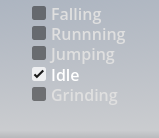
\includegraphics[width=\textwidth]{Images/UI_State_Idle.png}
	\end{minipage}
	\hfill
	\begin{minipage}{0.45\textwidth}
		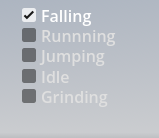
\includegraphics[width=\textwidth]{Images/UI_State_Fall.png}
	\end{minipage}
	\hfill
	\begin{minipage}{0.45\textwidth}
		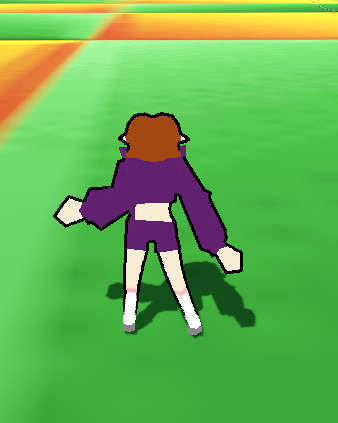
\includegraphics[width=\textwidth]{Images/Idle_State_IG.png}
		\caption{"Idle" állapot}
		\label{UI_Idle}
	\end{minipage}
	\hfill
	\begin{minipage}{0.45\textwidth}
		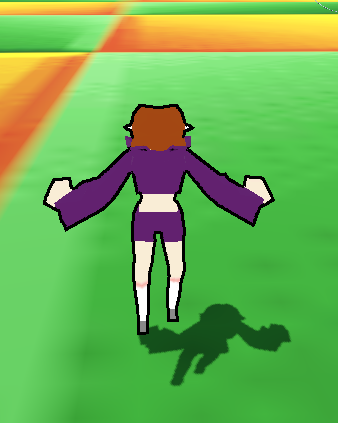
\includegraphics[width=\textwidth]{Images/Falling_State_IG.png}
		\caption{"Falling" állapot}
		\label{UI_Falling}
	\end{minipage}
\end{figure}


\section{Mozgásfunkciók tesztelése}

A mozgásfunkciókat csakis a színteren belül lehet teljes mértékben tesztelni, mivel szükséges látni, hogy a modell és a világ is jól reagál az inputokra. Egyedül az Idle állapot esetében nem fontos ez, mivel itt csak annyit kell tudnunk, hogy mozog-e (vagy éppen megállóban van-e) a karakterünk, minden más esetében elengedhetetlen a vizuális megjelenítés.

\begin{tabularx}{\textwidth}{ 
  | >{\raggedright\arraybackslash}X 
  | >{\raggedright\arraybackslash}X 
  | >{\raggedright\arraybackslash}X 
  | >{\raggedright\arraybackslash}X
  | >{\raggedright\arraybackslash}X |}
\hline
Teszteset & Kiinduló állapot & Bemenet / Esemény & Elvárt állapot & Eredmény\\
\hline
Állásból mozgás & Grounded / Idle & Movement Input & Running & sikeres\\
Mozgásból ugrás & Running & Jump Input & Jumping & sikeres\\
Levegőben mozgás & Jumping & Movement Input & InAir Movement & sikeres\\
Dupla ugrás & Falling & Jump Input & Jumping & sikeres\\
Landolás & Falling & No Input & Grounded / Idle & sikeres\\
Landolás után mozgás & Falling & Movement Input & Running & sikeres\\
Csúszás & Jumping / Sín közelébe érés & Automatikus amint érintkezik sínnel & Grinding & sikeres*\\
\hline
\end{tabularx}

\vspace{1cm}
*A csúsász esetében egyetlen küszöbproblémát vettem észre. Amikor a játékos modellje bizonyos szögekből való beérkezéskor rossz irányt vett fel. Ez magára a csúszás menetére ugyan nincsen kihatással, értsük ezt úgy, hogy a mozgás irányára és sebessége nem változik, viszont elvesz a játékélményből.

\section[Összegzés]{A tesztelés összegzése}

A próbák során a mozgásrendszert mindig nagyon élvezetes volt használni, soha nem fordult elő olyan eset, hogy beragadtam volna egy állapotba és mindig pontosan jelezve volt, hogy melyik állapotban voltam akkor. Az esés közben volt néha az, hogy úgy éreztem mint ha túl "lebegős" lenne, túl lassan esne a karakter, és a sebességnél a gyorsulás volt még néhány esetben furcsa, ezeket viszont a számok állítgatásával orvosolni lehet. Mindenesetre kijelenthetem, hogy tesztek sikeresek voltak és minden úgy működik, ahogy az elő volt írva.
